\documentclass{article}
\usepackage{unipr_org_notes}
% grafici
\usepackage{pgfplots}
\usepackage{float}
\usepackage[T1]{fontenc}
\usepackage{lmodern}
\usepackage{tikz}
\usepackage{multirow}

\usetikzlibrary{positioning, arrows.meta, shapes.geometric,backgrounds}


% --- colori per i grafici (th_03) ---
\definecolor{fn_bg}{HTML}{D9EAD3} % Sfondo verde chiaro per 'false negatives'
\definecolor{tn_bg}{HTML}{EFEFEF} % Sfondo grigio chiaro per 'true negatives'
\definecolor{tp_fill}{HTML}{B6D7A8} % Verde più scuro per 'true positives'
\definecolor{fp_fill}{HTML}{F4CCCC} % Rosso chiaro per 'false positives'
\definecolor{datapoint}{HTML}{666666} % Grigio per i punti
\definecolor{fn_area}{HTML}{8A9A83} % Verde/Grigio scuro per area 'relevant' (FN)
% ---------------------------------


% --- colori per i punti (th_04) ---
\definecolor{myblue}{RGB}{0, 0, 200}
\definecolor{mygreen}{RGB}{0, 170, 0}
\definecolor{myred}{RGB}{200, 0, 0}
% ---------------------------------

\renewcommand{\coursetitle}{Algoritmi per l'intelligenza artificiale}

% \addauthor{Nome}{Mail}


\renewcommand{\authorname}{Simone Colli}
% \renewcommand{\authoremail}{simone.colli@studenti.unipr.it}

\renewcommand{\notedate}{%
    Appunti del corso tenuto dal \textbf{Prof. Vincenzo Bonnici} \\
    \medskip % Aggiunge un piccolo spazio verticale
    Università degli Studi di Parma \\
    Anno Accademico 2025/2026
}


\begin{document}
\maketitle

\tableofcontents

%% blocco slide 1
\section{Introduzione}

Nel campo dell'apprendimento automatico classico,
le attività sono tradizionalmente suddivise in
quattro rami principali:
\begin{itemize}
    \item Apprendimento supervisionato (supervised).
    \item Apprendimento semi-supervisionato (semi-supervised).
    \item Apprendimento non supervisionato (unsupervised).
    \item Apprendimento per rinforzo (reinforcement learning).
\end{itemize}
La distinzione primaria tra queste metodologie di ML risiede nel
livello di disponibilità dei ``dati di verità di base'' (ground truth).
Il \textbf{ground truth} è definito come la conoscenza preliminare dell'output
che il modello dovrebbe produrre per un dato input, basata sull'osservazione
diretta in contrapposizione all'inferenza.

\subsection{Apprendimento automatico supervisionato}

L'apprendimento automatico supervisionato ha come obiettivo l'apprendimento di
una funzione che, dato un \textbf{campione di dati} e i relativi output desiderati,
riesca ad approssimare la funzione sottostante che mappa gli input agli output.
Questa metodologia è comunemente applicata in due principali contesti:
\begin{itemize}
    \item \textbf{Classificazione}: quando si desidera mappare l'input a
    etichette di output discrete.
    \item \textbf{Regressione}: quando l'obiettivo è mappare l'input a un
    output continuo.
\end{itemize}
In entrambi i casi, lo scopo è identificare relazioni o strutture specifiche
nei dati di input che consentano di generare output corretti in modo efficace.
È fondamentale notare che la correttezza dell'output è determinata interamente
dai dati di addestramento, i quali costituiscono la ``verità di base'' che il
modello apprende.

L'efficacia del modello può essere significativamente ridotta dalla
presenza di etichette ``rumorose'' o ``errate'' all'interno dei dati stessi.
Algoritmi notevoli nell'apprendimento supervisionato includono la regressione
logistica, il classificatore bayesiano naif, le macchine a vettori di supporto,
le reti neurali artificiali e le foreste casuali.
Il successo di un modello di ML dipende dalla sua capacità di
generalizzazione. Questo concetto è strettamente connesso alla complessità del
modello, che si riferisce alla complessità della funzione che si sta cercando
di apprendere.
Se si dispone di una quantità limitata di dati o se questi non sono distribuiti
uniformemente, è cruciale optare per un modello a bassa complessità per evitare
situazioni di overfitting.

L'\textbf{overfitting} (sovradattamento) si verifica quando il modello apprende la funzione adattandosi
troppo bene ai soli dati di addestramento, senza cogliere la tendenza o la
struttura effettiva che guida l'output, e quindi non riesce a generalizzare
a nuovi punti dati.
La gestione della generalizzazione è formalizzata tramite il compromesso
\textbf{bias-varianza} (bias-variance tradeoff).
Così facendo il modello presenterà un equilibrio tra:
\begin{itemize}
    \item \textbf{Bias} (distorsione): l'errore sistematico dovuto a ipotesi errate nel
    processo di apprendimento.
    \item \textbf{Varianza}: la quantità in base alla quale l'errore può
    variare tra diversi set di dati.
\end{itemize}
La difficoltà si presenta nel creare un modello che cattura accuratamente le
regolarità dei dati di addestramento e che sia in grado di generalizzare bene
a dati non visti in precedenza.
Generalmente, un aumento del bias (e una conseguente riduzione della
varianza) porta a modelli con livelli di prestazione più stabili e
garantiti, un fattore che può essere cruciale in certe applicazioni.
Per ottenere una buona generalizzazione, la varianza del
modello deve essere attentamente bilanciata in base alla dimensione e
alla complessità dei dati di addestramento.

\begin{nota}{Gestione dei dataset}{}
    Set di dati piccoli e semplici dovrebbero essere gestiti con modelli a
    bassa varianza, mentre set di dati grandi e complessi richiedono
    modelli con una varianza più elevata per poter catturare appieno la
    struttura sottostante dei dati.
\end{nota}

\subsection{Apprendimento automatico semi-supervisionato}

L'apprendimento automatico semi-supervisionato (semi-supervised)
mira a \textbf{etichettare i punti dati senza etichetta}
sfruttando la conoscenza appresa da un piccolo numero di dati già etichettati.
Metodi comuni includono le \textbf{macchine vettoriali di supporto
trasversali} e i \textbf{metodi basati su grafi} (come la
propagazione delle etichette).
\begin{nota}{Vantaggi dell'apprendimento semi-supervisionato}{}
    L'apprendimento semi-supervisionato può migliorare significativamente
    le prestazioni del modello rispetto all'apprendimento supervisionato
    quando si dispone di una quantità limitata di dati etichettati.
    La quantità di dati etichettati limitata si può presentare in
    diversi scenari, come ad esempio:
    \begin{itemize}
        \item Dati etichettati costosi da ottenere (ad esempio, richiedono
        l'intervento umano).
        \item Dati etichettati difficili da ottenere (ad esempio, richiedono
        competenze specialistiche).
        \item Dati etichettati soggetti a vincoli di privacy o etici.
    \end{itemize}
\end{nota}

\begin{esempio}{Rilevamento di messaggi inappropriati}{}
    Nel rilevamento di messaggi inappropriati in un social network,
    è impraticabile etichettare manualmente ogni messaggio.
    Si può, invece, etichettare manualmente un piccolo sottoinsieme
    e usare tecniche semi-supervisionate per comprendere e classificare
    il resto dei contenuti.
\end{esempio}

\subsubsection{Presupposti dell'apprendimento semi-supervisionato}

Per poter giustificare l'utilizzo di pochi dati etichettati per trarre
conclusioni su un grande insieme di dati non etichettati, i metodi
semi-supervisionati si basano su alcuni presupposti fondamentali, quali:
\begin{itemize}
    \item \textbf{Continuità}: Si assume che punti dati ``vicini'' tra
    loro abbiano maggiori probabilità di condividere la stessa
    etichetta.
    \item \textbf{Ipotesi del cluster}: Si presume che i dati formino
    naturalmente dei cluster discreti. Di conseguenza,
    punti nello stesso cluster hanno maggiori probabilità di
    condividere un'etichetta.
    \item \textbf{Presupposto molteplice (manifold)}: Si ipotizza che
    i dati si trovino approssimativamente in uno spazio di
    dimensioni inferiori (un \textit{manifold}) rispetto allo
    spazio di input originale. Questo è rilevante
    quando un sistema con pochi parametri, non osservabile
    direttamente, produce output osservabili ad alta
    dimensione.
\end{itemize}

\subsection{Apprendimento automatico non supervisionato}

L'apprendimento automatico non supervisionato (unsupervised)
opera \textbf{senza output etichettati}. L'obiettivo principale
di questa tecnica è quello di \textbf{dedurre la
struttura naturale} presente all'interno di un insieme di dati,
cercando di trovare \textbf{pattern} intrinseci
nei dati. Le attività più comuni in questo ambito includono:
\begin{itemize}
    \item \textbf{Clustering} (raggruppamento).
    \item \textbf{Apprendimento della rappresentazione}
    (representation learning).
    \item \textbf{Stima della densità} (density estimation).
\end{itemize}
In tutti questi casi, si desidera comprendere la struttura
intrinseca dei dati senza usare etichette fornite
esplicitamente.
Tecniche comuni includono il \textbf{clustering}, l'analisi
dei componenti principali (\textbf{PCA}) e gli \textbf{autocodificatori}
(autoencoders). Le due principali sono il clustering
e la riduzione della dimensionalità dei dati.

\begin{nota}{Valutazione delle prestazioni}{}
Dato che non vengono fornite etichette, nella maggior parte
dei metodi di apprendimento non supervisionato non esiste un
modo specifico per confrontare le prestazioni del modello.
\end{nota}

\subsubsection{Clustering}

Il clustering è una \textbf{tecnica esplorativa} che permette di
aggregare dati in gruppi (detti \textit{cluster}) senza avere
una precedente conoscenza della loro appartenenza a tali
gruppi. Si applica a dataset dove i dati al loro
interno presentano elementi simili tra loro.
All'interno di ogni singolo cluster si troveranno quindi dati
che hanno molte \textbf{caratteristiche simili} tra loro.
È un'ottima tecnica per trovare relazioni tra i dati.

\subsubsection{Riduzione della dimensionalità}

La riduzione della dimensionalità senza supervisione è un
approccio molto usato nella \textbf{pre-elaborazione delle
features}. L'obiettivo principale di questa tecnica è
di \textbf{eliminare il ``rumore''} dai dati.
Un altro utilizzo si trova nella \textbf{rappresentazione dei dati}:
dati in uno spazio delle caratteristiche ad elevata dimensionalità
possono essere proiettati su uno spazio 1D, 2D o 3D per
l'analisi visiva.

\begin{nota}{Compromesso tra riduzione della dimensionalità e prestazioni}{}
    Questa operazione può talvolta causare una minore prestazione predittiva.
    Ma può anche rendere lo spazio dimensionale più compatto, aiutando a
    \textbf{mantenere le informazioni più rilevanti}.
\end{nota}

\subsubsection{Analisi esplorativa}

L'apprendimento non supervisionato è estremamente utile
nell'\textbf{analisi esplorativa dei dati} (exploratory data
analysis), poiché è in grado di \textbf{identificare
automaticamente la struttura} nei dati.
Ad esempio, se un analista volesse segmentare i consumatori,
i metodi di clustering sarebbero un ottimo punto di partenza
per l'analisi.

In situazioni dove è impraticabile o impossibile per un essere
umano proporre tendenze nei dati, l'apprendimento non
supervisionato può fornire \textbf{informazioni iniziali} che
possono poi essere usate per testare o verificare singole
ipotesi.

\subsection{Apprendimento per rinforzo}

L'apprendimento con rinforzo (reinforcement learning) ha l'obiettivo di
realizzare \textbf{agenti autonomi}. Questi agenti devono
essere in grado di scegliere azioni da compiere per conseguire
determinati obiettivi. Questo avviene tramite
l'interazione con l'ambiente in cui sono immersi, con lo scopo
di massimizzare una nozione di \textbf{premio cumulativo}.

%% blocco slide 2
\section{Classificazione}

La classificazione è un'attività dell'apprendimento supervisionato che
consiste nell'assegnare un'etichetta (o classe) a un dato
sulla base di sue caratteristiche osservabili.
Nell'ambito della classificazione si parla di:
\begin{itemize}
    \item \textbf{Feature} (caratteristica): un aspetto direttamente
    osservabile di un fenomeno per il quale si può registrare una
    misura, che sia quantitativa (numerica) o categoriale
    (come vero/falso, rosso/verde, ecc..).
    \item \textbf{Classe}: un concetto astratto
    e generale che ``spiega'' le osservazioni. L'assegnazione
    a una classe costituisce una sintesi delle feature osservate.
    \item \textbf{Label} (etichetta): il nome specifico di una classe.
\end{itemize}

\begin{nota}{Problematica della classificazione}{}

    Alcuni dati possono rendere più complesso l'assegnazione delle classi.
    Questa tipologia di dati è nota come \textbf{outlier statistici}.

\end{nota}

\begin{definizione}{Collezione di dati}{def:collezione_dati}
    Una collezione di dati è un insieme di elementi $P$ di $M$-uple
    del tipo:
    \[
    m_i = (x_{1i}, \ldots, x_{Mi}) \in D_1 \times \ldots \times D_M
    \]
    dove ogni $x_{ji}$ rappresenta una feature ed appartiene ad un possibile
    dominio di valori $D_j$.
    Ogni feature $x_{ji}$ appartiene a un dominio di valori $D_j$.
    I domini possono essere:
    \begin{itemize}
        \item \textbf{Numerici:} (es. $\mathbb{R}$ per valori continui,
        $\mathbb{Z}$ per discreti).
        \item \textbf{Categoriali:} Insiemi finiti di valori (es.
        \{Rosso, Verde, Blu\}).
    \end{itemize}
\end{definizione}

\begin{definizione}{Partizionamento in classi }{def:partizionamento_classi}
Data una collezione di dati \Cref{def:collezione_dati} $P$ e
un insieme finito di $k$ \textbf{etichette} (o classi) $L = \{A_1, \ldots, A_k\}$.

Si dice che $P$ è \textbf{partizionato in classi} se $P$ è suddiviso in
$k$ sottoinsiemi $\{C_1, \ldots, C_k\}$, tali che:
\begin{itemize}
    \item $C_j \subseteq P$, $\forall j \in \{1, \ldots, k\}$
    \item $C_i \cap C_j = \emptyset$, $\forall i \neq j$ (le classi sono
    mutuamente esclusive)
    \item $\bigcup_{j=1}^k C_j = P$ (l'unione delle classi copre l'intero dataset)
\end{itemize}
Ogni sottoinsieme $C_j$ raggruppa tutti e soli gli elementi $m_i \in P$
che sono stati associati all'etichetta (classe) $A_j \in L$.
\end{definizione}

\begin{definizione}{Algoritmo di classificazione}{def:alg_classificazione}
Un \textbf{algoritmo di classificazione} è una funzione computabile
$f: P \mapsto L$, tale che:
\[
f(m \in P) = f(x_1, \ldots, x_m) \in L
\]
Tale funzione $f(m)$ assegna a ogni dato $m$ un'etichetta $A_i$ scelta
tra quelle presenti in $L$ cercando di stimare l'etichetta reale del stesso.

Lo schema di classificazione può produrre due tipi di risultati:
\begin{itemize}
    \item \textbf{Successo} (hit) se l'etichetta stimata $f(m)$
    coincide con l'etichetta reale del dato.
    \item \textbf{Fallimento} (miss) se l'etichetta stimata è errata.
\end{itemize}

\end{definizione}

\begin{nota}{Classificatori \textit{error free}}{}
È generalmente impossibile creare classificatori \textit{error free}.
Per questo motivo è fondamentale fornire stime sul tasso percentuale di
hit/miss.

Il livello tollerabile di errore dipende dalla \textbf{criticità
dell'applicazione}: per applicazioni industriali si può richiedere un
tasso $< 5\%$, mentre per applicazioni mediche un tasso $> 0.5\%$
potrebbe essere già inaccettabile.
\end{nota}

\begin{esempio}{Problema di classificazione: salmoni e branzino}{ex:salmoni_branzino}

Si consideri il problema di distinguere tra salmoni e branzini (sea bass) basandosi
su alcune caratteristiche osservabili.
Le \textbf{feature} utilizzate potrebbero essere la lunghezza, il peso in grammi
e il colore dominante (un attributo qualitativo scelto da un insieme predefinito
come \{blu, grigio, verde\}).
I dati vengono tipicamente organizzati in una tabella, dove ogni riga corrisponde
a un pesce e le colonne ne descrivono le feature.

L'obiettivo è costruire un classificatore che, per ogni nuovo pesce osservato,
sia in grado di riempire la colonna ``specie'' con l'etichetta corretta
(``salmone'' o ``branzino'').
È importante notare che gli errori non hanno lo stesso costo: confondere un
salmone (pesce pregiato) con un branzino (meno pregiato) è un errore più grave
del contrario.

\end{esempio}

\begin{esempio}{Problema di classificazione: studenti e carriera}{ex:studenti_carriera}

Si consideri il problema di predire il futuro successo economico degli studenti
universitari.
Le \textbf{feature} raccolte per ogni studente includono dati anagrafici, il
censo familiare e i voti conseguiti durante la carriera universitaria.
L'obiettivo è costruire un classificatore che predica in quale \textbf{classe}
di reddito si troverà lo studente dieci anni dopo la laurea. Le etichette
(o \textbf{label}) potrebbero essere \{``reddito basso'', ``reddito medio'',
``reddito alto''\}.

È importante notare che, a causa dell'elevato numero di fattori non misurabili
che influenzano la vita di un individuo, una predizione del genere ha un valore
limitato se applicata al singolo studente, che ha un'alta probabilità di essere
classificato erroneamente.

Tuttavia, questo tipo di analisi è estremamente utile a livello statistico e
aggregato, per comprendere le tendenze generali di un'intera popolazione
studentesca e informare politiche educative o economiche.

\end{esempio}

\subsection{Costruire un classificatore}

Il processo di costruzione di un classificatore automatico simula
il fenomeno dell'apprendimento umano o animale, noto come
\textbf{training} (addestramento). L'idea è \textbf{dedurre regole
generali}, applicabili a record non ancora classificati,
partendo dall'osservazione di esempi già noti e ben classificati.

Gli algoritmi e le tecniche di classificazione automatica sono
numerosissimi. Tutti i metodi noti condividono uno \textbf{schema
generale} (Figura \ref{fig:th_02_01}) ben testato e riconosciuto dalla comunità scientifica.

\begin{figure}[H]
    \centering
    \includegraphics[width=0.6\textwidth]{images/th_02/01.png}
    \caption{Schema generale di un sistema di classificazione}
    \label{fig:th_02_01}
\end{figure}

\begin{definizione}{Universo delle osservazioni}{def:universo_osservazioni}
    Si definisce \textbf{universo delle osservazioni} l'insieme
    complessivo dei record (passati, presenti e futuri) relativi ad un fenomeno.
    Molti algoritmi iniziano esaminando un sottoinsieme di questo
    universo, già classificato e ben compreso.
\end{definizione}

Un universo delle osservazioni \Cref{def:universo_osservazioni} 
che rappresenta l'insieme di ``allenamento'', chiamato \textbf{Training Set
(TS)}, è il deposito di informazioni iniziali da cui l'algoritmo
ricava le ``regole'' di classificazione. Le regole ricavate saranno di vario
tipo: statistiche, probabilistiche, fuzzy, funzioni discendenti, ecc.

\subsection{Proprietà di un classificatore}

Un buon insieme di regole di classificazione deve avere tre
importanti proprietà:
\begin{itemize}
    \item \textbf{Semplicità}: Le regole non devono essere troppo
    complicate, per garantire efficienza e basso costo computazionale
    in fase di classificazione.
    \item \textbf{Correttezza sul TS}: Le regole devono essere
    statisticamente sufficientemente corrette quando applicate
    al medesimo Training Set che le ha generate.
    \item \textbf{Generalizzabilità}: Le regole devono essere
    statisticamente corrette anche quando applicate al resto
    dei record dell'universo (dati nuovi, non visti).
\end{itemize}

\begin{nota}{}{}
Il termine \textbf{statisticamente corretto} su un training set indica che il
tasso dei miss non deve superare certe soglie di tolleranza che dipendono
dalla criticità delle applicazioni.
\end{nota}

\subsection{Il problema dell'overfitting}

Le proprietà di correttezza sul TS e di generalizzabilità sono
spesso in conflitto tra loro.
Questo paradosso è noto come \textbf{overfitting} (sovradattamento).
L'overfitting si verifica quando un modello si adatta
``troppo bene'' ai dati del Training Set. Un modello molto
complesso può imparare a memoria le peculiarità e persino
il rumore casuale presente nel TS, ottenendo una correttezza
perfetta su di esso.
Tuttavia, tale modello non avrà appreso la ``tendenza'' generale
dei dati e fallirà nel generalizzare a nuovi record,
poiché la frontiera di decisione che ha appreso è
eccessivamente complessa e specifica per il campione di training.

L'obiettivo non è minimizzare l'errore sul TS (che
porterebbe a un modello complesso e in overfitting), ma
trovare un equilibrio: un modello (es. una retta o una
curva semplice) che, pur commettendo qualche errore sul TS,
catturi la struttura di fondo dei dati e possa quindi
generalizzare meglio.

\subsection{Validazione}

Per ``convalidare'' la proprietà di generalizzazione di un
insieme di regole, si utilizza un metodo che prevede, oltre
al TS, un altro insieme di record già etichettati, detto
\textbf{Control Set (CS)} o \textbf{Test Set}.
Il CS \textbf{non} viene utilizzato durante la fase di
training (cioè per la sintesi delle regole). Viene usato
solo dopo che le regole sono state definite.
Se le regole mostrano sul CS un tasso di errore (miss)
simile a quello ottenuto sul TS, allora si ritiene
che le regole siano \textbf{generalizzabili}.

Poiché anche il CS è un campione casuale, per una stima
più precisa è buona norma ripetere i test con diversi CS,
spesso creati tramite strategie di randomizzazione
nella selezione del TS e del CS dall'universo disponibile.

\subsection{Gestione delle feature e del rumore}

Nella costruzione di un classificatore è cruciale gestire
sia la selezione delle feature che la presenza di rumore.

\subsubsection{Selezione delle feature}
Spesso si rilevano molte feature, ma non tutte sono utili;
alcune possono essere sovrabbondanti o addirittura dannose.
Combinare più feature (es. lunghezza e luminosità dei pesci)
è spesso una strategia conveniente, ma non è detto che
sia sempre la migliore.
L'inclusione di troppe feature, specialmente se irrilevanti,
può amplificare il \"rumore\" e confondere il classificatore.
Una buona pratica è scegliere feature che siano
\textbf{invarianti} alle trasformazioni tipiche della
situazione sperimentale (es. il peso di un pesce è
invariante alle condizioni di luce, la luminanza no).
Inoltre, deve esistere una probabile relazione tra le
feature misurate e la classe da predire.

\subsubsection{Rumore e outlier}
I dati del mondo reale contengono inevitabilmente
\textbf{rumore}, ovvero perturbazioni dovute a fenomeni
non controllabili o non noti. Le cause di tale
spostamento dai valori ``ideali'' possono essere:
\begin{itemize}
    \item \textbf{Endogene}: Interne al fenomeno (es. un pesce
    con una dieta o storia anomala).
    \item \textbf{Esogene}: Dovute all'osservatore o allo
    strumento utilizzato (es. macchina fotografica starata,
    etichettatore distratto).
\end{itemize}

I dati molto ``fuori norma'' rispetto ai valori tipici di una
classe sono definiti \textbf{outlier}.
Un buon algoritmo di classificazione deve essere
\textbf{robusto}, ovvero deve avere una forma di
``protezione'' o resistenza alle deviazioni che il rumore
impone al processo decisionale.

\subsection{Valutazione degli errori}

Contare gli errori è essenziale, ma una singola percentuale
di errore non è sufficientemente descrittiva. Questo perché
non tutti gli errori sono uguali: i \textbf{costi degli errori}
spesso \textbf{non sono uniformi} o simmetrici.

Ad esempio, in una diagnosi medica:
\begin{itemize}
    \item Classificare un sano come malato (Falso Positivo)
    è un errore con un costo relativamente basso (paura, un
    test aggiuntivo).
    \item Classificare un malato come sano (Falso Negativo)
    è un errore gravissimo, che ritarda la diagnosi e
    può costare la vita al paziente.
\end{itemize}

Per analizzare questa asimmetria si usa la
\textbf{matrice di confusione}. È una griglia quadrata
che riporta quante istanze della classe ``reale'' (sulle colonne)
sono state assegnate alla classe ``prevista'' (sulle righe).

\begin{nota}{Matrice di confusione ideale}{}
    Un classificatore perfetto ha come matrice di confusione la
    matrice identica (tutti i valori sulla diagonale principale,
    zero altrove). Un buon classificatore avrà valori
    percentuali bassi al di fuori della diagonale principale.

\end{nota}
\subsection{Fasi di un sistema di classificazione}

Il processo di classificazione automatica si articola in
diverse fasi:
\begin{enumerate}
    \item \textbf{Sensing (o sampling)}: Raccolta dei dati dal
    mondo fisico e loro digitalizzazione.
    \item \textbf{Segmentazione}: Partizione dei dati in unità
    significative, pulizia ed eliminazione di dati irrilevanti.
    \item \textbf{Estrazione delle feature}: Misurazione delle
    caratteristiche (quantitative o qualitative). È cruciale
    scegliere feature invarianti e rilevanti.
    \item \textbf{Classificazione}: Esecuzione dell'algoritmo
    scelto per l'assegnazione delle etichette.
    \item \textbf{Post-processing}: Valutazione della qualità
    della classificazione e dei costi associati agli errori.
    \item \textbf{Decisione}: Utilizzo effettivo del
    classificatore per risolvere il problema reale.
\end{enumerate}

La costruzione di un classificatore è un \textbf{ciclo
iterativo} che prevede la raccolta dei dati, la selezione
delle feature, la scelta di un modello matematico, il
training dell'algoritmo e infine la sua valutazione,
ripetendo i passi per migliorare le prestazioni.
%% blocco slide 3


\section{Tecniche di validazione per la classificazione}

Dopo aver costruito un modello di classificazione, è fondamentale valutarne le
performance. A differenza della regressione, dove si cerca di predire un
valore numerico di output dato uno o più valori di input, nella
classificazione si vuole predire la classe di un oggetto dato uno o più
dati di input di qualsiasi tipo (numerici, categorici, testuali, ecc.).

Per questo motivo gli strumenti che si possono applicare per valutare un modello di
classificazione sono sostanzialmente diversi rispetto alle metriche utilizzate
per valutare i modelli di regressione.

\subsection{Modello di validazione base: Training e Test Set}

L'approccio base per la validazione consiste nel dividere, secondo una certa
\textbf{percentuale} i dati disponibili in due insiemi:

\begin{itemize}
    \item \textbf{Training set (TS)}: Utilizzato per addestrare il
    classificatore. Le etichette (label) di questi dati sono usate per
    addestrare il classificatore.
    \item \textbf{Test set}: Utilizzato per valutare la bontà del modello.
    Le etichette di questo set vengono usate solo per verificare se
    il classificatore ha predetto correttamente.
\end{itemize}

L'obiettivo della validazione non è solo misurare l'errore, ma ha lo scopo di
rispondere a domande più complesse, come:
\begin{itemize}
    \item Il classificatore performa in modo bilanciato su tutte le classi?
    \item Ha delle preferenze?
    \item Tali preferenze da cosa dipendono?
\end{itemize}
Per questo motivo per la valutazione dei classificatori si utilizzano indici
matematici che permettono sia di avere stime oggettive delle performance, sia
di automatizzare anche altre fasi del processo della progettazione o sviluppo
del classificatore.

Gli indici principali relativamente all'aspetto computazionale utilizzati
per valutare un classificatore sono:
\begin{itemize}
    \item \textbf{Accuratezza}: La bontà nel predire correttamente le
    etichette.
    \item \textbf{Robustezza}: La capacità di gestire dati con rumore o valori
    mancanti.
    \item \textbf{Velocità}: Include sia il tempo per costruire il modello
    (training time) sia il tempo per usarlo (classification/prediction time).
    \item \textbf{Scalabilità}: L'efficienza del modello su grandi dataset,
    specialmente se in memoria secondaria.
    \item \textbf{Interpretabilità}: La facilità con cui i risultati del
    modello possono essere compresi.
\end{itemize}

\subsection{Metriche di valutazione}
Per definire le metriche più comuni, si assume un problema di classificazione
binaria. Si assume che l'insieme delle classi $\mathbb{C}$ dell'esperimento
sia composto da due classi: $\mathbb{C}=\{A,B\}$.

Relativamente ad una delle classi è possibile definire alcune misure per
calcolare la bontà dell'algoritmo in valutare tale classe.

Data una classe di interesse (es. A, la classe ``positiva''),
i risultati della classificazione sul test set vengono divisi in quattro
categorie:

\begin{itemize}
    \item True positive (TP).
    \item True negative (TN).
    \item False positive (FP).
    \item False negative (FN).
\end{itemize}

\begin{center}
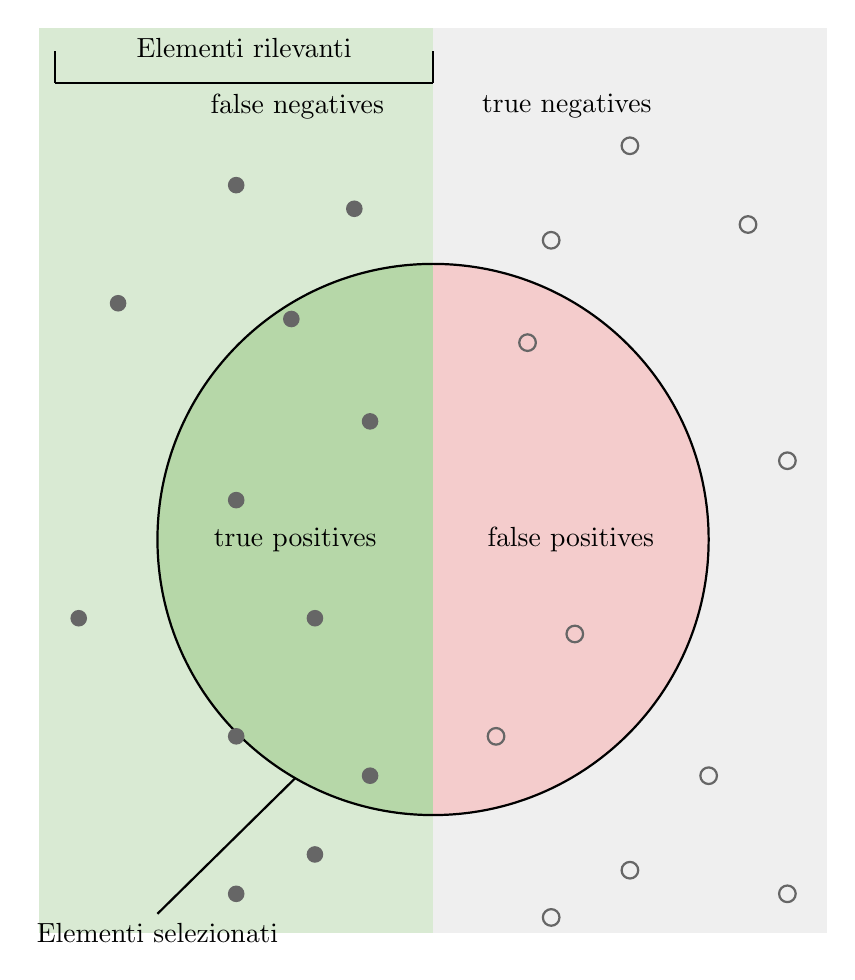
\begin{tikzpicture}[
    % Definiamo stili per i punti dati
    solid_point/.style = {
        circle, 
        fill=datapoint, 
        minimum size=6pt, 
        inner sep=0
    },
    hollow_point/.style = {
        circle, 
        draw=datapoint, 
        thick, 
        minimum size=6pt, 
        inner sep=0
    }
]

% 1. Disegnare le aree di sfondo (Actual)
% Sfondo per\"Relevant\"(Sinistra)
\fill[fn_bg] (-5, -5) rectangle (0, 6.5);
% Sfondo per\"Not Relevant\"(Destra)
\fill[tn_bg] (0, -5) rectangle (5, 6.5);

% 2. Disegnare il cerchio (Selected) e riempirlo
% Riempiamo la metà sinistra (True Positives)
\fill[tp_fill] (90:3.5) arc (90:270:3.5) -- cycle;
% Riempiamo la metà destra (False Positives)
\fill[fp_fill] (90:3.5) arc (90:-90:3.5) -- cycle;

% Disegniamo il bordo nero del cerchio
\draw[thick] (0, 0) circle (3.5cm);

% 3. Posizionare i punti dati
% False Negatives (Solidi, Sinistra, Fuori)
\node[solid_point] at (-2.5, 4.5) {};
\node[solid_point] at (-1, 4.2) {};
\node[solid_point] at (-4, 3) {};
\node[solid_point] at (-4.5, -1) {};
\node[solid_point] at (-2.5, -4.5) {};
\node[solid_point] at (-1.5, -4) {};

% True Positives (Solidi, Sinistra, Dentro)
\node[solid_point] at (-1.8, 2.8) {};
\node[solid_point] at (-0.8, 1.5) {};
\node[solid_point] at (-2.5, 0.5) {};
\node[solid_point] at (-1.5, -1) {};
\node[solid_point] at (-2.5, -2.5) {};
\node[solid_point] at (-0.8, -3) {};

% False Positives (Vuoti, Destra, Dentro)
\node[hollow_point] at (1.2, 2.5) {};
\node[hollow_point] at (1.8, -1.2) {};
\node[hollow_point] at (0.8, -2.5) {};

% True Negatives (Vuoti, Destra, Fuori)
\node[hollow_point] at (2.5, 5) {};
\node[hollow_point] at (4, 4) {};
\node[hollow_point] at (1.5, 3.8) {};
\node[hollow_point] at (4.5, 1) {};
\node[hollow_point] at (3.5, -3) {};
\node[hollow_point] at (2.5, -4.2) {};
\node[hollow_point] at (1.5, -4.8) {};
\node[hollow_point] at (4.5, -4.5) {};

% 4. Aggiungere le etichette
% Etichette di sfondo
\node[anchor=west] at (0.5, 5.5) {true negatives};
\node[anchor=east] at (-0.5, 5.5) {false negatives};

% Etichette del cerchio
\node at (-1.75, 0) {true positives};
\node at (1.75, 0) {false positives};

% Etichetta\"relevant elements\"con la staffa
\draw [thick] (-4.8, 6.2) -- (-4.8, 5.8);
\draw [thick] (-4.8, 5.8) -- (0, 5.8);
\draw [thick] (0, 5.8) -- (0, 6.2);
\node at (-2.4, 5.8) [above=2mm] {Elementi rilevanti};

% Etichetta\"selected elements\"con il puntatore
\node (label_sel) at (-3.5, -5) {Elementi selezionati};
% Il punto sul cerchio è a 240 gradi, raggio 3.5
\draw [thick, -] (label_sel.north) -- (240:3.5);

\end{tikzpicture}
\end{center}

\begin{definizione}{TP, TN, FP, FN}{}

Sia $c: CS \mapsto \mathbb{C}$ la funzione che mappa ogni record $x \in CS$
nella sua classe reale e sia $\tilde{c}: CS \mapsto \mathbb{C}$ il
classificatore che assegna una classe ad $A$.

Sia $C = \{A, B\}$ l'insieme delle classi, composto dalle classi $A$ e $B$.
Prendendo come riferimento la classe $A$ è possibile dividere $CS$ in 4 insiemi:

\begin{itemize}
    \item \textbf{True positive (TP)}: I record $x \in CS$ classificati \textbf{correttamente},
    ovvero la cui classe reale è $A$, quindi $\tilde{c}(x) = c(x) = A$
    \item \textbf{True negative (TN)}: I record $x \in CS$ classificati \textbf{correttamente},
    ovvero la cui classe reale è $B$, quindi $\tilde{c}(x) = c(x) = B$
    \item \textbf{False positive (FP)}: I record $x \in CS$ classificati \textbf{erroneamente},
    ovvero la cui classe reale è $B$, quindi $\tilde{c}(x) = B \ne A = c(x)$
    \item \textbf{False negative (FN)}: I record $x \in CS$ classificati \textbf{erroneamente},
    ovvero la cui classe reale è $B$, quindi $\tilde{c}(x) = A \ne B = c(x)$
\end{itemize}
\end{definizione}

\bigskip
Basandosi su queste quattro categorie, è possibile definire le metriche di
performance più utilizzate.

\begin{definizione}{Precision}{}
Sia $C = \{A, B\}$ l'insieme delle classi, composto dalle classi $A$ e $B$.
La precision (precisione) è la frazione di elementi rilevanti per una classe
di riferimento, $A$, tra tutti gli elementi che il classificatore ha
identificato come $A$.
La precision misura quanto è ``affidabile'' la predizione positiva,
ed è definita come:
\[
Precision = \frac{TP}{TP+FP}
\]

\end{definizione}

\begin{definizione}{Recall}{}
Sia $C = \{A, B\}$ l'insieme delle classi, composto dalle classi $A$ e $B$.
La recall (richiamo o sensitività) è la frazione di elementi rilevanti
(classi A) che sono stati correttamente classificati come A.
Misura la capacità del classificatore di ``trovare'' tutti i positivi.
\[
Recall = \frac{TP}{TP+FN}
\]
\end{definizione}

\begin{center}
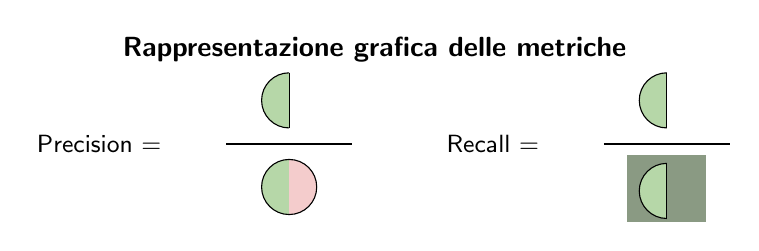
\begin{tikzpicture}[
    font=\sffamily\small,
    radius=0.35cm % Raggio ridotto per i cerchi
]

% --- Titolo ---
\node[font=\sffamily\bfseries] at (3.5, 1.2) {Rappresentazione grafica delle metriche};


% --- Definiamo una forma riutilizzabile per il semicerchio TP ---
\def\tpsemicircle{
    % Arrotondamento verde
    \fill[tp_fill] (90:0.35) arc (90:270:0.35) -- cycle;
    % Bordo dell'arco
    \draw[black] (90:0.35) arc (90:270:0.35);
    % Linea dritta
    \draw[black] (90:0.35) -- (270:0.35);
}

% --- 1. Precision ---
% Etichetta
\node (prec_label) at (0, 0) {Precision =};

% Posizioniamo la frazione a destra dell'etichetta
\begin{scope}[shift={(prec_label.east)}, xshift=1.5cm]
    
    % Numeratore (TP Semicerchio)
    \begin{scope}[yshift=0.55cm]
        \tpsemicircle
    \end{scope}
    
    % Linea di frazione
    \draw[thick] (-0.8, 0) -- (0.8, 0);
    
    % Denominatore (TP + FP Cerchio intero, "selected elements")
    \begin{scope}[yshift=-0.55cm]
        \fill[tp_fill] (90:0.35) arc (90:270:0.35) -- cycle;
        \fill[fp_fill] (90:0.35) arc (90:-90:0.35) -- cycle;
        \draw[black] (0,0) circle (0.35);
    \end{scope}
\end{scope}

% --- 2. Recall ---
% Etichetta
\node (rec_label) at (5, 0) {Recall =};

% Posizioniamo la frazione a destra dell'etichetta
\begin{scope}[shift={(rec_label.east)}, xshift=1.5cm]
    
    % Numeratore (TP Semicerchio)
    \begin{scope}[yshift=0.55cm]
        \tpsemicircle
    \end{scope}
    
    % Linea di frazione
    \draw[thick] (-0.8, 0) -- (0.8, 0);
    
    % Denominatore (Come da tua immagine: Rettangolo scuro [FN] che contiene TP)
    % Questo rappresenta (TP) / (TP + FN) o "relevant elements"
    \begin{scope}[yshift=-0.85cm]
        % Rettangolo scuro di sfondo (FN)
        \fill[fn_area] (-0.5, -0.15) rectangle (0.5, 0.7);
        % Semicerchio TP sovrapposto
        \begin{scope}[yshift=0.25cm]
            \tpsemicircle
        \end{scope}
    \end{scope}
\end{scope}

\end{tikzpicture}
\end{center}

\begin{nota}{Valori ottenuti}{}
Valori alti per entrambe le metriche indicano un buon classificatore.
Spesso, però, si preferisce utilizzare un indice unico che le combini.
\end{nota}
\bigskip
\begin{definizione}{$F_1$-Score}{}
Il $F_1$-Score rappresenta la media armonica di precision e recall.
Fornisce un equilibrio tra le due metriche.
\[
F_{1} = 2 \cdot \frac{Precision \cdot Recall}{Precision + Recall}
      = \frac{2 \cdot TP}{2 \cdot TP + FP + FN}
\]
Come precision e recall, anche l'$F_1$-Score ha un valore compreso tra 0 e 1.
Maggiore è il valore, maggiore è la bontà del classificatore.
\end{definizione}

\begin{nota}{Overfitting}{}
Sebbene un $F_1$-Score alto sia desiderabile, valori molto prossimi a 1
possono essere un campanello d'allarme per l'overfitting.
\end{nota}

\subsection{Accuracy}

\begin{definizione}{Accuracy}{}
La accuracy (accuratezza) misura la quantità totale di oggetti classificati
correttamente (sia positivi che negativi) rispetto al totale degli oggetti.
\[
Accuracy = \frac{TP+TN}{TP+TN+FP+FN}
\]
\end{definizione}

\begin{nota}{Accuratezza per dataset sbilanciati}{}
L'accuracy standard è poco indicata se le classi non sono bilanciate.
Ad esempio, in un dataset con 95 campioni negativi e 5 positivi,
un classificatore ``pigro'' che predice sempre ``negativo'' otterrebbe un'accuratezza
del 95\%, pur essendo totalmente inutile nel riconoscere i positivi.
\end{nota}

In situazione di sbilanciamento delle classi, si preferisce la Balanced accuracy.

\begin{definizione}{Balanced accuracy}{}
La Balanced accuracy (accuratezza bilanciata) è la media tra la sensitività
(per i positivi) e la specificità (per i negativi).
\[
Balanced\ accuracy = \frac{TPR + TNR}{2}
\]
dove:
\begin{itemize}
    \item \textbf{TPR (True Positive Rate)}: È la Recall/Sensitività:
    $TPR = \frac{TP}{TP+FN}$.
    \item \textbf{TNR (True Negative Rate)}: È la Specificità:
    $TNR = \frac{TN}{TN+FP}$.
\end{itemize}
\end{definizione}

\subsection{Altri indici e matrice di confusione}

\begin{definizione}{False Discovery Rate (FDR)}{}
Misura il tasso di errori di tipo I (``false scoperte'' o Falsi positivi)
rispetto a tutte le predizioni positive.
\[
FDR = \frac{FP}{FP+TP} = 1 - Precision
\]
\end{definizione}

\subsubsection{Matrice di confusione}
La matrice di confusione è una tabella che riassume le performance di un
classificatore binario, incrociando le classi reali con quelle predette e
mostrando i conteggi di TP, TN, FP e FN.
È fondamentale perché non tutti gli errori hanno lo stesso costo, come
discusso in precedenza (es. diagnosi medica errata).

\begin{figure}[H]
    \centering
    \includegraphics[width=0.6\textwidth]{images/th_03/01.png}
    \caption{Esempio di matrice di confusione per classificazione binaria.}
\end{figure}

È importante notare che metriche come sensitività, precisione e specificità
dipendono dalla classe presa in considerazione, mentre l'accuratezza è un
indice globale.

\subsection{Area Under the Curve (AUC) e curva ROC}

L'AUC (Area Under the Curve) è una misura basata sulla curva ROC (Receiver
Operating Characteristics).

\begin{definizione}{Curva ROC}{}
Una curva ROC è un grafico che mostra le performance di un classificatore
al variare di un suo parametro (es. una soglia). Mette in relazione il
\textbf{True Positive Rate (TPR)} (sull'asse Y) con il \textbf{False Positive
Rate (FPR)} (sull'asse X).

( $FPR = 1 - Specificit\grave{a} = \frac{FP}{FP+TN}$ ).

Le curve ROC passano sempre per i punti $(0,0)$ e $(1,1)$. Esistono inoltre due
condizioni limite che rappresentano due curve di riferimento:

\begin{itemize}
    \item Una retta che taglia il grafico a 45 gradi passando per l'origine.
    Questa retta rappresenta il caso del \textbf{classificatore casuale} e
    l'area sottesa (AUC) è pari a $0.5$.
    \item Una curva rappresentata dal segmento che dall'origine sale
    verticalmente al punto $(0,1)$ e dal segmento che congiunge il punto
    $(0,1)$ a $(1,1)$. Questa curva ha un'area sottesa di valore pari a 1 e
    rappresenta il \textbf{classificatore perfetto}.
\end{itemize}
\end{definizione}


L'AUC, ha un valore compreso tra 0 e 1, e misura l'intera area bidimensionale
sotto la curva ROC.
\begin{itemize}
    \item \textbf{AUC = 1}: Rappresenta il classificatore perfetto, che
    passa per il punto (0,1)
    \item \textbf{AUC = 0.5}: Rappresenta il classificatore casuale
    (la linea diagonale).
    \item \textbf{AUC = 0}: Rappresenta il classificatore
    ``perfettamente sbagliato'' (che inverte tutte le predizioni).
\end{itemize}
Il valore di AUC (tra 0 e 1) può essere interpretato come la probabilità
che il classificatore assegni un punteggio più alto a un individuo positivo
scelto a caso, rispetto a un individuo negativo scelto a caso.

\subsection{Classificazione multi-classe}

Le misure viste finora (Precision, Recall, $F_1$-score) sono definite per la
classificazione binaria. Per applicarle a problemi con $K > 2$ classi, si
perde la visione di performance globale.
Per l'$F_1$-score, si possono calcolare delle medie. L'approccio
comune è ``one-vs-rest'': per ogni classe $g_i \in G = \{ 1, \ldots, K \}$,
si costruisce una matrice di confusione dove $g_i$ è il ``caso positivo'' e
tutte le altre classi formano il ``caso negativo''.
Si calcolano così $TP_i$, $FP_i$ e $FN_i$ per ogni classe $i$.

\subsubsection{Micro-average}
La micro-average (micro-media) aggrega i contributi di tutte le classi
``sull'unità più piccola'' (i singoli campioni) prima di calcolare le
metriche.
Queste metriche sono:
\[
P_{micro}=\frac{\sum_{i=1}^{|G|}TP_{i}}{\sum_{i=1}^{|G|}(TP_{i}+FP_{i})}
\]
\[
R_{micro}=\frac{\sum_{i=1}^{|G|}TP_{i}}{\sum_{i=1}^{|G|}(TP_{i}+FN_{i})}
\]
Da cui si può derivare il $F_1$-score micro-averaged, $F_{1_{micro}}$
che rappresenta la media armonica di $P_{micro}$ e $R_{micro}$.

\[
F_{1_{micro}} = 2 \cdot \frac{P_{micro} \cdot R_{micro}}{P_{micro} + R_{micro}}
\]

\begin{nota}{Micro-average e classi sbilanciate}{}
Questa misura non è sensibile alle prestazioni sulle singole classi e può
essere fuorviante se la distribuzione delle classi è sbilanciata.
\end{nota}

\subsubsection{Macro-average}
La macro-average (macro-media) calcola la media su gruppi più vasti.
\[
P_{macro}=\frac{\sum_{i=1}^{|G|}P_{i}}{|G|}
\]
\[
R_{macro}=\frac{\sum_{i=1}^{|G|}R_{i}}{|G|}
\]
Da cui si può derivare il $F_1$-score macro-averaged, $F_{1_{macro}}$
che rappresenta la media armonica di $P_{macro}$ e $R_{macro}$.
\[
F_{1_{macro}} = 2 \cdot \frac{P_{macro} \cdot R_{macro}}{P_{macro} + R_{macro}}
\]

\begin{nota}{Macro-average per dati sbilanciati}{}
Se questo valore è grande, indica che il classificatore funziona bene
(in media) per ogni singola classe.
Per questo motivo è più adatto per dati con distribuzione sbilanciata.
\end{nota}

\subsubsection{Generalizzazione di AUC (Metodo Hand \& Till)}
Esiste anche una generalizzazione dell'AUC per $k > 2$ classi (Metodo Hand
\& Till, 2001).
L'idea è calcolare una misura di separabilità $\hat{A}(i|j)$
per ogni possibile coppia di classi $(i, j)$.

\begin{definizione}{Generalizzazione AUC}{}

Sia $\hat{A}(i|j)$ la probabilità che dato un elemento a caso della classe $j$
abbia probabilità inferiore di attribuire quell'elemento alla classe $i$,
rispetto al valore di probabilità che attribuirebbe ad un elemento a caso
della classe $i$.
È possibile calcolare $\hat{A}(i|j)$ utilizzando le seguenti definizioni:
\begin{itemize}
    \item $\hat{p}(X_l)$ è la probabilità stimata che l'osservazione $l$ sia
    originata dalla classe $i$.
    \item per tutte le osservazioni $x_l$ della classe $i$, sia $f_l = \hat{p}(X_l)$.
    la probabilità stimata di appartenere alla classe $i$.
    \item per tutte le osservazioni $x_k$ della classe $j$, sia $g_k = \hat{p}(X_k)$.
    la probabilità stimata di appartenere alla classe $i$.
\end{itemize}

Allora i valori ottenuti ordinati in modo crescente sono:
$\{g_1, \ldots, g_n, f_1, \ldots, f_n\}$.
Sia $r_{l}$ il rango della $l$-esima osservazione della classe $i$.

Il numero totale di coppie di punti in cui il punto della classe $j$ ha
un valore di probabilità stimato di appartenenza alla classe $i$ inferiore
a quello della classe $i$ è:
\[
\sum_{l=1}^{N_i} (r_l - l) = \sum_{l=1}^{N_i} r_l - \sum_{l=1}^{N_i} l = S_i - \frac{N_i(N_i+1)}{2}
\]
Dove $N_i$ e $N_j$ sono il numero di osservazioni delle classi $i$ e $j$ e
$S_i$ è la somma dei ranghi delle osservazioni della classe $i$.

La probabilità che un punto scelto a caso della classe $j$ abbia una probabilità
stimata di appartenenza alla classe $i$ inferiore a quella di un punto
scelto a caso della classe $i$ è quindi:
\[
\hat{A}(i|j) = \frac{S_i - \frac{N_i(N_i+1)}{2}}{N_i \cdot N_j}
\]

Inoltre considerando che non è possibile distinguere $\hat{A}(i | j)$ da
$\hat{A}(j | i)$, si ha che la misura di separabilità tra le classi $i$ e $j$
è data dalla media tra $\hat{A}(i | j)$ e $\hat{A}(j | i)$, ovvero:
\[
\hat{A}(i|j) = \frac{\hat{A}(i|j) + \hat{A}(j|i)}{2}
\]

Il valore di AUC globale ($M$) di un classificatore multi-classe è quindi dato
dalla media di tutti i valori $\hat{A}(i|j)$ calcolati è definito come:
\[
M=\frac{2}{c(c-1)}\sum_{i<j}\hat{A}(i|j)
\]
Dove $c$ è il numero totale di classi, $\frac{2}{c(c-1)}$
è un fattore che viene applicato perchè sono presenti $c(c-1)$ modi
differenti con cui costruire coppie distinte di classi.

\end{definizione}

\subsection{Cross-validation}

\begin{definizione}{Cross-Validazione}{}
È una tecnica statistica usata per validare un modello e valutare come
i suoi risultati si generalizzeranno a un insieme di dati indipendente.
L'obiettivo primario è testare la capacità del modello di prevedere su nuovi
dati, non usati durante l'addestramento.
Serve principalmente a stimare problemi di \textbf{overfitting} o di
\textbf{selection bias}.
\end{definizione}

Il \textit{selection bias} si verifica quando la scelta del training
set è viziata (da fattori esterni) e non rispecchia un campionamento
uniforme dell'universo delle osservazioni.

\begin{nota}{Selection bias}
Il \textit{selection bias} può portare a stime distorte delle performance
del modello, poiché il training set non rappresenta adeguatamente la
popolazione generale.
È importante essere consapevoli di questo bias durante la fase di
progettazione dello studio e nella raccolta dei dati.

Training set e test set dovrebbero essere prodotti tramite campionamento
uniforme dell'universo delle possibili osservazioni.
\end{nota}

La cross-validazione si divide in due tipi principali:
\begin{itemize}
    \item Cross-validazione esaustiva, che testa tutte le possibili divisioni
    del dataset in TS e CS.
    \item Cross-validazione non esaustiva, che testa solo un sottoinsieme delle
    possibili divisioni.
\end{itemize}

\subsubsection{Cross-validazione esaustiva}
La cross-validazione esaustiva testa tutti i modi possibili di dividere il dataset in TS e CS.
\begin{itemize}
    \item \textbf{Leave-p-out (LPO)}: Utilizza $p$ osservazioni come
    CS e $N-p$ come TS. Questo processo viene ripetuto per tutti le
    $\binom{n}{p}$ possibili combinazioni.
    \item \textbf{Leave-one-out (LOOCV)}: È un caso particolare di LPO
    dove $p=1$. È appropriata per dataset molto piccoli, dove il
    costo computazionale è secondario rispetto all'accuratezza della stima.
\end{itemize}

\subsubsection{Cross-validazione non esaustiva}

La cross-validazione non esaustiva testa solo un sottoinsieme
delle possibili divisioni.
La tecnica più comune è la \textbf{k-fold cross-validation}, dove il dataset
viene diviso casualmente in $k$ parti (fold) di eguale dimensione.
A turno, ogni ``fold'' viene usato come Test Set (CS) e i restanti
$k-1$ fold vengono usati come Training Set (TS).
Il processo si ripete $k$ volte e le metriche vengono mediate.
%% blocco slide 4
\section{Algoritmi di classificazione}

\subsection{Tipologie di modelli di classificazione}

I modelli di classificazione possono essere suddivisi in due tipologie:
\begin{itemize}
    \item \textbf{Eager (volenterosi)}: Costruiscono un modello generale e
    indipendente dall'input a partire dai dati di addestramento.
    Tale modello viene poi usato per classificare nuovi dati.
    \item \textbf{Lazy (pigri)}: Memorizzano semplicemente i dati di
    addestramento (in forma grezza o con piccole elaborazioni) e rimandano
    l'intero processo di classificazione all'arrivo della nuova
    istanza da classificare.
\end{itemize}

In generale, i metodi lazy richiedono meno tempo in fase di addestramento ma
molto più tempo in fase di classificazione.
Riguardo l'accuratezza, i metodi lazy usano uno spazio delle ipotesi più ricco,
potendo usare funzioni locali di classificazione che forniscono approssimazioni
a livello globale.
Al contrario, i metodi eager si riferiscono a una sola ipotesi per coprire
l'intero universo delle osservazioni.

Approcci tipicamente lazy includono:
\begin{itemize}
    \item \textbf{k-nearest neighbors (kNN)} (i k vicini più prossimi): I
    data point sono rappresentati in uno spazio euclideo.
    \item \textbf{Locally weighted regression}: Costruisce approssimazioni
    locali.
    \item \textbf{Case-based reasoning}: Usa rappresentazione simbolica e
    inferenza basata sulla conoscenza (knowledge-based inference).
\end{itemize}

\subsection{k-Nearest Neighbors (kNN)}

Nel kNN, l'insieme delle osservazioni è rappresentato come un insieme di data
point in uno spazio $n$-dimensionale, dove ogni dimensione può avere valori
reali o discreti.

Lo spazio è tipicamente euclideo (su cui si calcolano distanze euclidee),
ma è possibile utilizzare anche feature categoriali con metriche diverse
(es. Jaccard, Tanimoto, Dice, Hamming, distanza al coseno).

\begin{definizione}{k-Nearest Neighbors (kNN)}
Dato un training set (TS) e un'istanza da classificare, l'algoritmo assegna a
tale istanza la classe che è più rappresentata tra i suoi \textbf{k} vicini
più prossimi.

\begin{center}
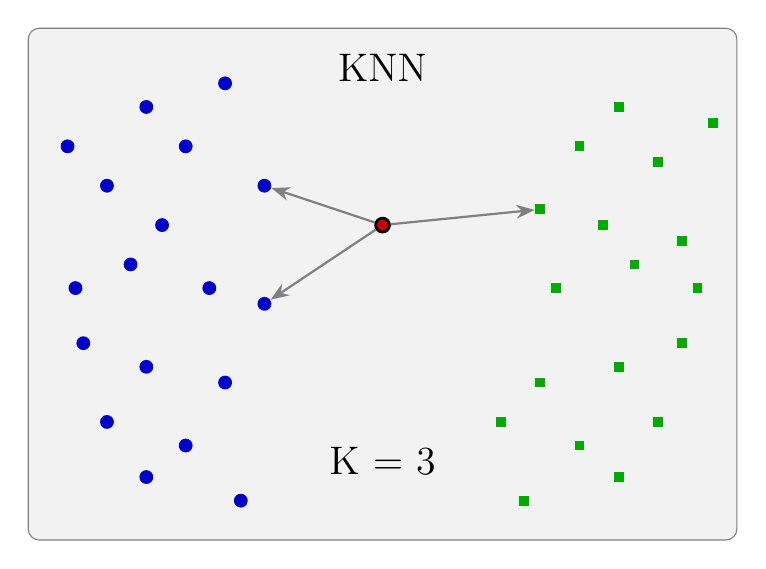
\begin{tikzpicture}[
    % --- Definiamo stili per i nodi ---
    point/.style={minimum size=5pt, inner sep=0},
    blue_point/.style={point, circle, fill=myblue},
    green_point/.style={point, regular polygon, regular polygon sides=4, fill=mygreen},
    red_point/.style={point, circle, fill=myred, line width=1pt, draw=black}
]

% 1. Disegnare il riquadro esterno
\draw[draw=gray, fill=gray!10, rounded corners] (-4.5, -3) rectangle (4.5, 3.5);

% 2. Aggiungere i titoli
\node at (0, 3) {\Large KNN};
\node at (0, -2) {\Large K = 3};

% 3. Posizionare il punto da classificare (rosso)
% Lo chiamiamo 'query' per poterlo referenziare
\node (query) [red_point] at (0, 1) {};

% 4. Posizionare i 3 vicini più prossimi (K=3)
\node (b_near_1) [blue_point] at (-1.5, 1.5) {};
\node (b_near_2) [blue_point] at (-1.5, 0) {};
\node (g_near_1) [green_point] at (2, 1.2) {};

% 5. Disegnare le frecce dal punto 'query' ai vicini
\draw[->, thick, gray, -Stealth] (query) -- (b_near_1);
\draw[->, thick, gray, -Stealth] (query) -- (b_near_2);
\draw[->, thick, gray, -Stealth] (query) -- (g_near_1);

% 6. Posizionare tutti gli altri punti (cluster)
% --- Cluster Blu ---
\node [blue_point] at (-3, 2.5) {};
\node [blue_point] at (-2.5, 2) {};
\node [blue_point] at (-3.5, 1.5) {};
\node [blue_point] at (-2.8, 1) {};
\node [blue_point] at (-3.2, 0.5) {};
\node [blue_point] at (-2.2, 0.2) {};
\node [blue_point] at (-3.8, -0.5) {};
\node [blue_point] at (-3, -0.8) {};
\node [blue_point] at (-2, -1) {};
\node [blue_point] at (-3.5, -1.5) {};
\node [blue_point] at (-2.5, -1.8) {};
\node [blue_point] at (-1.8, -2.5) {};
\node [blue_point] at (-3.0, -2.2) {};
\node [blue_point] at (-3.9, 0.2) {};
\node [blue_point] at (-4.0, 2.0) {};
\node [blue_point] at (-2.0, 2.8) {};

% --- Cluster Verde ---
\node [green_point] at (3, 2.5) {};
\node [green_point] at (2.5, 2) {};
\node [green_point] at (3.5, 1.8) {};
\node [green_point] at (2.8, 1) {};
\node [green_point] at (3.2, 0.5) {};
\node [green_point] at (2.2, 0.2) {};
\node [green_point] at (3.8, -0.5) {};
\node [green_point] at (3, -0.8) {};
\node [green_point] at (2, -1) {};
\node [green_point] at (3.5, -1.5) {};
\node [green_point] at (2.5, -1.8) {};
\node [green_point] at (1.8, -2.5) {};
\node [green_point] at (3.0, -2.2) {};
\node [green_point] at (4.0, 0.2) {};
\node [green_point] at (1.5, -1.5) {};
\node [green_point] at (3.8, 0.8) {};
\node [green_point] at (4.2, 2.3) {};
\end{tikzpicture}
\end{center}

\end{definizione}

\begin{nota}{Il ruolo di k}{}
    Il parametro $k$ è un punto chiave dell'algoritmo perché determina il
    numero di vicini da considerare per la classificazione.
\end{nota}

Il kNN è uno strumento \textbf{non parametrico}, cioè non fa alcuna ipotesi
sulla distribuzione dei dati.
Questo è utile perché la maggior parte dei dati ``reali'' non obbedisce ad
assunti teorici (come nei modelli di regressione lineare).

Di conseguenza, kNN è spesso una delle prime scelte per uno studio di
classificazione quando c'è poca o nessuna conoscenza sulla distribuzione
dei dati.

\subsubsection{Potere predittivo e scelta di k}
Il potere predittivo dipende dal parametro $k$:
\begin{itemize}
    \item \textbf{k piccolo}: Limita la regione di previsione, rendendo il
    classificatore ``più cieco'' alla distribuzione generale.
    \item \textbf{k grande}: Riduce l'impatto della varianza e dell'errore
    casuale, ma rischia di ignorare piccoli dettagli rilevanti.
\end{itemize}

Alcuni autori suggeriscono di impostare $k$ uguale alla radice quadrata del
numero di osservazioni nel training set.
Un'alternativa migliore è usare la cross-validazione per identificare il
valore di $k$ con le performance migliori.

\subsubsection{Weighted kNN}
Per migliorare le performance, si può usare una versione pesata (Weighted kNN),
dove le classi dei vicini sono pesate in base alla loro distanza.
Ad esempio, si può pesare l'apporto di ogni vicino con l'inverso della sua
distanza ($1/d_i$).

\begin{nota}{Weighted kNN e dataset sbilanciati}{}
Per dataset sbilanciati, si può anche pesare l'apporto di ogni vicino con
l'inverso del numero totale di punti nel dataset aventi la stessa classe del
vicino in questione.
\end{nota}

\subsection{Alberi di decisione}

\begin{definizione}{Albero di decisione}
Un albero di decisione descrive un albero di ricerca (n-ario) dove i nodi
foglia rappresentano le classificazioni e le ramificazioni l'insieme delle
proprietà che portano a quelle classificazioni.
Ogni nodo interno contiene un test (tipicamente su una feature o una
combinazione di feature) che stabilisce quale sotto-albero deve essere
visitato.
\end{definizione}

\subsubsection{Costruzione dell'albero}
L'algoritmo di costruzione (top-down, greedy) inizia con un nodo radice che
contiene tutti i dati di addestramento e segue una strategia ricorsiva:
\begin{enumerate}
    \item Se tutti i dati di training in un nodo $t$ hanno lo stesso valore
    sull'attributo classificatore, si crea un nodo foglia contenente
    tutti i dati.
    \item Altrimenti, si cerca la partizione $S$ degli elementi (basata su
    un attributo) che massimizza una misura di ``goodness'' (purezza).
    \item Si sceglie la partizione $S^*$ che massimizza la misura di
    ``goodness''.
    \item Si creano tanti figli del nodo $t$ quante sono le classi/valori
    presenti in $S^*$.
    \item Un nodo figlio è detto ``puro'' se tutti i suoi elementi hanno lo
    stesso valore di classe.
    \item Si applica ricorsivamente l'algoritmo sui nodi impuri (o che non
    rappresentano una singola classe secondo una soglia di maggioranza).
\end{enumerate}

L'obiettivo è scegliere l'albero più semplice a parità di performance e il più
compatto possibile. Trovare l'ipotesi minimale è NP-hard, per cui si usa
questa strategia greedy (divide-et-impera) che non garantisce l'ottimalità.

La decisione principale è scegliere l'attributo su cui biforcare in modo che
divida in insiemi il più puri possibile e porti rapidamente a nodi foglia.

\subsubsection{Goodness functions}

Le misure di ``goodness'' (purezza) più utilizzate per scegliere l'attributo
migliore per lo split sono:
\begin{itemize}
    \item \textbf{Information Gain (ID3, C4.5)}: Basato sulla riduzione
    dell'entropia. Adatto per attributi categoriali (ma modificabile per
    i continui).
    \item \textbf{Indice di Gini (CART)}: Adatto per attributi continui,
    assume che esistano diversi valori di splitting per ogni attributo
    (tipicamente split binari).
\end{itemize}

\subsubsection{Information gain}

La scelta basata sull'\textbf{information gain} mira alla riduzione
progressiva dell'entropia.
L'entropia $H$ misura il disordine (o l'incertezza media) di una variabile
aleatoria.

\[
H(p_1, \ldots, p_k) = -\sum_{i}p_{i}\log_{b}p_{i}
\]
L'entropia è massima quando tutti gli eventi sono equiprobabili (massimo
disordine).

Dato un insieme $S$ con $k$ classi $C_i$, l'informazione (entropia)
necessaria per classificare un campione in $S$ misura la \textbf{quantità di
informazione media necessaria} ed è definita come:
\[
Info(S) = -\sum_{i=1}^{k}\frac{freq(C_{i},S)}{|S|}\log_{2}\frac{freq(C_{i},S)}{|S|}
\]

Se si partiziona $S$ usando un attributo $A$ (con $n$ valori) nei sottoinsiemi
$\{S_1, \ldots, S_n\}$, l'entropia dell'albero con radice $A$ è la media ponderata
delle entropie dei sottoinsiemi:
\[
Info_{A}(S) = \sum_{i=1}^{n}\frac{|S_{i}|}{|S|}Info(S_{i})
\]

La quantità di informazione guadagnata dal partizionamento di $S$
è la riduzione dell'entropia ottenuta splittando sull'attributo $A$:
\[
Gain(A) = Info(S) - Info_{A}(S)
\]
L'algoritmo seleziona l'attributo $A$ che massimizza il
$Gain(A)$ (o, equivalentemente, minimizza $Info_A(S)$).

\begin{esempio}{Information gain con due classi}
Sia $C$ l'insieme delle classi con due classi $C_1$ e $C_2$, e sia
$S$ un insieme che contiene $c_1$ elementi di $C_1$ e $c_2$ elementi di $C_2$.

La \textbf{quantità di informazione} necessaria per decidere se un elemento
arbitrario in $S$ appartiene a $C_1$ o $C_2$ è:
\[
Info(c_1, c_2) = -\frac{c_1}{c_1 + c_2}\log_{2}\frac{c_1}{c_1 + c_2}
- \frac{c_2}{c_1 + c_2}\log_{2}\frac{c_2}{c_1 + c_2}
\]

Assumendo di utilizzare un attributo $A$ con $v$ valori $\{a_1, a_2, \ldots, a_v\}$,
come radice dell'albero, allora $S$ viene partizionato in $v$ sottoinsiemi
$\{S_1, S_2, \ldots, S_v\}$.

Così facendo $C_1$ e $C_2$ si dividono in $\{[C_1]_1, [C_1]_2, \ldots, [C_1]_v\}$ e
$\{[C_2]_1, [C_2]_2, \ldots, [C_2]_v\}$.

Se $S_i$ contiene $[c_{1}]_i$ elementi di $C_1$ e $[c_2]_i$ elementi di $C_2$,
allora la quantità di informazione richiesta per classificare gli oggetti nei
vari $S_i$ saranno $Info([c_{1}]_i, [c_{2}]_i)$.

Di conseguenza l'informazione richiesta per l'albero con radice $A$ sarà la
media pesata dagli $Info$ secondo le partizioni che $A$ impone su $S$:
\[
Info_{A}(S) = \sum_{i=1}^{v}\frac{[c_1]_i + [c_2]_i}{c_1 + c_2} Info([c_{1}]_i, [c_{2}]_i)
\]

\end{esempio}

\begin{nota}{Sbilanciamento dell'Information Gain}{}
L'Information gain è fortemente sbilanciato in favore dei test che hanno molti
esiti (es. un attributo ID), anche se questi esiti sono poco significativi
in termini di predizione.
Come soluzione a questa problematica si normalizza il gain in base alla
quantità di informazione ottibile da $S$ stesso.

Considerando l'\textbf{informazione} contenuta da un messaggio sulla probabile
partizione di $S$ in $S_i$ insiemi, si ha che tale informazione è data da:
\[
-\log_{2}\frac{|S_{i}|}{|S|}
\]

Per analogia la definizion di $Info(S)$ è porta alla definizione di
$SplitInfo$, che rappresenta la potenziale informazione generata dalla
divisione di $S$.
\[
SplitInfo(A) = -\sum_{i=1}^{n}\frac{|S_{i}|}{|S|}\log_{2}\frac{|S_{i}|}{|S|}
\]

Il \textbf{gain normalizzato}, ottenuto usando $SplitInfo$, è quindi:
\[
GainRatio(A) = \frac{Gain(A)}{SplitInfo(A)}
\]

Il GainRatio non risolve tutti i problemi, infatti potrebbe succedere che
attributi significativi assumono un qualche valore in più rispetto agli altri
risultando svantaggiati.

Una strategia comune è:
\begin{enumerate}
    \item Calcolare il $Gain(A)$ per ogni attributo.
    \item Calcolare la media dei guadagni.
    \item Selezionare \textbf{solo} gli attributi con guadagno sopra la media.
    \item Scegliere, tra gli attributi selezionati, quello con $GainRatio$ maggiore.
\end{enumerate}

\end{nota}


\begin{nota}{Attributi continui}{}
Per attributi di tipo continuo, si valuta l'utilizzo di un valore di soglia
$Z$, che rende il test binario: $A > Z$ o $A \le Z$.

Si testano tutti i possibili valori di soglia $v_j$ (o i punti medi tra valori
ordinati) presenti nel training set e si sceglie la soglia che massimizza il
gain.
Così facendo l'insieme di dati viene diviso in due sottoinsiemi $\{v_1, v_2,
\ldots, v_i\}$ e $\{v_{i+1}, v_{i+2}, \ldots, v_m\}$.

Questo critero va ad introdurre implicitamente un'altra restizione, richiedendo
che gli insiemi generati abbiano almeno un certo numero minimo di elementi.
\end{nota}

\begin{nota}{Gestione dei valori mancanti}{}

Durante la costruzione dell'albero, può capitare che alcuni record
abbiano valori mancanti (nulli) per alcuni attributi.
Tra le varie opzioni per gestire questi casi, si possono usare varie strategie:
\begin{itemize}
    \item Assegnare il valore più comune per quell'attributo.
    \item Assegnare una probabilità a ognuno dei possibili valori.
    \item Attribuire un peso ai record.
\end{itemize}

In queste situazioni è necessario adattare il calcolo del $Gain(A)$:
\[
Gain(A) = F \cdot (Info(S) - Info_A(S))
\]
dove $F$ è la percentuale di casi nel training set in cui l'attributo $A$ è
noto.

La variazione sul calcolo del $Gain(A)$ può essere estesa anche al calcolo
della $SplitInfo(A)$, e di conseguenza del $GainRatio(A)$, influendo così
sul partizionamento.

\bigskip

Per pesare i singoli record, è necessario valutare che se un record ha un
valore sconosciuto il peso è proprio la probabilità che il valore sia $v_i$.
Ogni sottoinsieme $S_i$ è una collezione di casi con pesi possibilmente
frazionali, così che $|S_i|$ può essere reinterpretata come la somma dei
pesi frazionali dei casi del sottoinsieme.

In generale, un caso di $S$ con peso $w$ il cui esito non è noto a ogni
sotto insieme $S_i$ con peso $w^*$ ha la probabilità che l'esito sia $v_i$

\end{nota}


\subsubsection{Indice di Gini}

\begin{definizione}{Indice di Gini}{}

L'indice di Gini è una metrica utilizzata per valutare la purezza dei nodi e
guidare la costruzione degli alberi.
Questa misura l'impurità di un insieme $S$.

Dato un insieme $S$ con $n$ classi, l'\textbf{indice di Gini} è definito come:
\[
gini(S) = 1 - \sum_{j=1}^{n}p_{j}^{2}
\]
dove $p_j$ è la frequenza della classe $j$:

Definito questo è necessario adattare il calcolo dello split basato su Gini,
definendo l'\textbf{indice di impurità dello split} come segue:
\[
gini_{split}(S, A) = \sum_{i=1}^{m}\frac{N_{i}}{N}gini(S_{i})
\]
dove $S$ è diviso in $m$ sottoinsiemi $S_i$ (di dimensione $N_i$) in base
all'attributo $A$, e $N = \sum_{i=1}^{m} N_i$ è la dimensione totale di $S$.

\end{definizione}


\begin{esempio}{Indice di Gini con due classi}{}

Date due classi $P$ e $N$, tale che $S = P \cup N$, contenenti rispettivamente
$p$ e $n$ elementi, è possibile calcolare:
\[
p_p = \frac{p}{p + n}
\]
\[
p_n = \frac{n}{p + n}
\]
\[
gini(S) = 1 - p_{p}^{2} - p_{n}^{2}
\]

Da questo si può calcolare l'indice di Gini per lo split su un attributo
$A$ che divide $S$ in due sottoinsiemi $S_1$ e $S_2$, rispettivamente con
dimensioni $N_1$ e $N_2$.

\[
gini_{split}(S, A) = \frac{N_1}{N}gini(S_1) + \frac{N_2}{N}gini(S_2)
\]

\end{esempio}

\begin{nota}{Algoritmo di CART}{}

L'algoritmo CART (che usa Gini) seleziona l'attributo $a$ che ha il
\textbf{minore} $gini_{split}(S, a)$, in quanto si cerca la massima riduzione
dell'impurità. Per gli attributi numerici, CART testa tutti i possibili split
binari.

\end{nota}

\subsubsection{Pruning}
Un albero cresciuto molto in profondità rischia di adattarsi troppo ai dati di
training, inclusi gli outlier e il rumore. Questa situazione è detta
\textbf{overfitting} e porta a un aumento degli errori su dati nuovi.

La soluzione è il \textbf{pruning} (potatura), ovvero la rimozione di parti
dell'albero (rami) che non contribuiscono significativamente alla
classificazione corretta, producendo un modello meno complesso e più
generalizzabile.

Le strategie di pruning sono:
\begin{itemize}
    \item \textbf{Pre-pruning}: Attuato durante la costruzione. Si decide di
    non dividere ulteriormente un nodo se il gain è inferiore a una soglia
    $t$, o se la purezza è già sufficiente (es. tramite metodi statistici).
    \item \textbf{Post-pruning}: Attuato dopo la costruzione completa
    dell'albero. Si recidono rami analizzando l'impatto sull'errore (spesso
    su un validation set). È più dispendioso ma generalmente più efficace
    (C4.5 usa il post-pruning).
\end{itemize}

\begin{nota}{Potature e distribuzione di probabilità}{}
Quando si pota, la foglia risultante potrebbe non essere pura. Invece di una
classe, le si associa una distribuzione di probabilità delle classi presenti.
\end{nota}

\paragraph{C4.5}
C4.5 (Pessimistic Pruning) utilizza un post-pruning ``pessimistico'' basato sul
set di training stesso.
Stima l'errore di un sottoalbero e lo confronta con l'errore medio che si
otterrebbe sostituendo il sottoalbero con una singola foglia (o, in C4.5,
anche con uno dei suoi rami).
Se l'errore stimato del sottoalbero potato è minore, il nodo viene potato.

\paragraph{Minimal cost-complexity pruning}
CART (minimal cost-complexity pruning) è un algoritmo di potatura
parametrizzato da $\alpha \ge 0$ (parametro di complessità).

Si definisce un costo di complessità $R_{\alpha}(T)$ per un albero $T$ come:
\[
R_{\alpha}(T) = R(T) + \alpha |\tilde{T}|
\]
dove $R(T)$ è il tasso di errore (impurità) dell'albero e $|\tilde{T}|$ è
il numero di nodi terminali (foglie).
L'algoritmo cerca il sottoalbero che minimizza $R_{\alpha}(T)$.


Si calcola un $alpha$ effettivo, $\alpha_{eff}$ come seguente:
\begin{itemize}
    \item Se il nodo $t$ è una foglia, $R_{\alpha}(T_t) = R(t)$.
    \item Altrimenti, per un nodo non terminale:
    \[
    \alpha_{eff} = \frac{R(t) - R(T_t)}{|T_t| - 1}
    \]
\end{itemize}
Si pota iterativamente il nodo non terminale con il $\alpha_{eff}$ più
piccolo.
All'aumentare di $\alpha$, l'albero viene potato di più,
l'impurità (errore sul training) aumenta, ma la generalizzazione
(errore sul test) migliora fino a un certo punto ottimale, per poi peggiorare
(underfitting).

\begin{figure}[H]
    \centering
    \includegraphics[width=0.6\textwidth]{images/th_04/01.png}
    \caption{All’aumentare di $\alpha$, viene potata una parte maggiore
    dell’albero, il che aumenta l’impurità totale delle sue foglie.}
\end{figure}

\begin{figure}[H]
    \centering
    \includegraphics[width=0.6\textwidth]{images/th_04/01.png}
    \caption{Il numero di nodi e la profondità dell’albero diminuiscono
    all’aumentare di $\alpha$}
\end{figure}

\begin{nota}{Valore di $\alpha$ e overfitting}{}
    Quando il valore di soglia è impostato a $0$ (nessuna potatura), l'albero
    va in overfitting, portando ad una precisione di allenamento del $100\%$
    ma ad una precisione di test dell' $80\%$.

    All'aumento di $\alpha$, viene tagliata una parte maggiore dell'albero,
    creando così un albero decisionale che generalizza meglio.

    \begin{figure}[H]
    \centering
    \includegraphics[width=0.6\textwidth]{images/th_04/03.png}
    \caption{Andamento dell’accuratezza in funzione di $\alpha$.}
    \end{figure}

\end{nota}
\subsection{Metodi consenso}

Gli alberi di decisione sono semplici e interpretabili, ma spesso non
competitivi in termini di qualità predittiva.
Inoltre, sono instabili, piccoli cambiamenti nei dati di training possono
portare a un albero molto diverso (alta varianza).

Per ovviare a questi svantaggi, si utilizzano differenti strategie tra cui
\textbf{bagging}, \textbf{random forests}, e \textbf{boosting}, che
costruiscono molteplici alberi e li combinano in un'unica predizione
\textbf{consenso}, migliorando notevolmente l'accuratezza a scapito (parziale)
dell'interpretabilità.

L'obiettivo è impiegare una combinazione di modelli $M^*$, ottenuta
combinando $k$ modelli addestrati separatamente, per incrementare
l'accuratezza. I metodi più popolari sono:
\begin{itemize}
    \item \textbf{Bagging}: Media la predizione su una collezione di
    classificatori.
    \item \textbf{Boosting}: Impiega una collezione di classificatori tramite
    un voto pesato.
    \item \textbf{Ensemble}: Combina un insieme eterogeneo di classificatori.
\end{itemize}

\subsubsection{Bagging}

Il bagging (Bootstrap Aggregation) è una tecnica generale per ridurre la
varianza di un metodo statistico, particolarmente utile per gli alberi
di decisione.

L'idea è simulare la disponibilità di più training set, anche se se ne ha
uno solo:
\begin{enumerate}
    \item Si estraggono $B$ diversi sottoinsiemi (campioni \textbf{bootstrap})
    dall'unico training set (estraendo casualmente con reinserimento).
    \item Si apprende un classificatore (un albero) $f_i$ per ciascun
    sottoinsieme $i$.
    \item Si aggregano (ensemble) le predizioni sulle nuove istanze $x$ di test:
    \[
    f_{bag}(x) = \frac{1}{B} \sum_{i=1}^{B} f_i(x)
    \]
\end{enumerate}


\subsubsection{Random Forest}
Una Random Forest è un metodo consenso costituito da un
\textbf{bagging di alberi di decisione non potati} (complessi), con
un'aggiunta cruciale: \textbf{una scelta casuale di un sottoinsieme delle
feature (predittori) ad ogni split}.

\begin{nota}{Metodologia}{}
    La random forest è un metodo non lineare (come gli alberi di decisione)
    e robusto, con bassa varianza e stabilità delle predizioni rispetto al
    variare dei dati di input.
    
    Migliora le prestazioni di un singolo albero di decisione appreso su
    tutti i dati ma perde la facile interpretabilità e scala meno bene.
\end{nota}

\paragraph{Addestramento della foresta}
Fissato un numero di alberi $n_{tree}$ e il numero di predittori (numero di
feature da testare a ogni split) $m_{try}$ da scegliere casualmente tra quelle
disponibili, viene ripetuto per $n_{tree}$ la procedura seguente:
\begin{enumerate}
    \item Si estrae un campione bootstrap $S$ dai dati di training.
    \item Si apprende un albero di decisione su $S$ accurato (minsplit = 1),
    in cui ad ogni split solo $m_{try}$ predittori sono scelti casualmente
    come candidati.
    \item Non viene effettuato il pruning.
    \item Si salva l'albero ottenuto tra quelli disponibili.
\end{enumerate}

\paragraph{Predizione}
Si aggregano le predizioni degli $n_{tree}$ alberi tramite voto di maggioranza
(classificazione) o media (regressione).

\begin{nota}{Scelta di $m_{try}$}{}
Di solito, $m_{try} \approx \sqrt{m}$ per la classificazione e
$m_{try} \approx m/3$ per la regressione (dove $m$ è il numero totale di
feature).
\end{nota}

\begin{nota}{Costruzione raffinata}{}
Il bagging riduce la varianza mediando alberi non distorti (perché profondi)
ma soggetti a errore (alta varianza).
La varianza di una media di $B$ variabili i.i.d. (indipendenti e identicamente
distribuite) con varianza $\sigma^2$ è $\frac{1}{B}\sigma^2$.

Tuttavia, gli alberi del bagging non sono indipendenti, perché crescono dallo
stesso TS (anche se bootstrapped).
Sono correlati. Se la correlazione a coppie è $\rho > 0$, la varianza della
media è:
\[
\rho\sigma^2 + \frac{1-\rho}{B}\sigma^2
\]
Al crescere di $B$, la varianza non va a zero, ma tende a $\rho\sigma^2$.

L'idea della Random Forest è \textbf{ridurre la correlazione $\rho$} tra gli
alberi. Introducendo la selezione casuale di $m_{try}$ feature ad ogni split,
si ``decorrelano'' gli alberi. Questo permette di migliorare la riduzione della
varianza del bagging, senza accrescere troppo la distorsione (bias).
\end{nota}

\paragraph{Valutazione (OOB error):}
Le RF forniscono una \textbf{stima dell'errore} di test chiamata
\textbf{Out-Of-Bag (OOB) error}.
Per ogni istanza di training $x_i$, si usano per la predizione solo gli alberi
che *non* contenevano $x_i$ nel loro campione bootstrap (circa 1/3 degli alberi).
L'OOB error è la media degli errori su queste predizioni.

\paragraph{Importanza delle features}

Si può stimare l'importanza di una feature in due modi:
\begin{itemize}
    \item \textbf{Mean decrease in accuracy (permutation importance)}: Si
    calcola l'accuratezza OOB. Poi, per una feature $i$, si permutano
    casualmente i suoi valori nei dati OOB (rompendo la correlazione con la
    classe). Si ricalcola l'accuratezza. La differenza media (su tutti gli
    alberi) nella precisione è l'importanza di quella feature.
    \item \textbf{Mean decrease in Gini index:} Si misura quanto lo split su
    una certa variabile riduce (in media) l'impurità (indice di Gini)
    attraverso tutti gli alberi.
\end{itemize}


\begin{nota}{Vantaggi}{}
Le random forest (RF) presentano diversi vantaggi chiave rispetto ai singoli alberi
decisionali:
\begin{itemize}
    \item \textbf{Scalabilità}: La complessità temporale aumenta in modo
    contenuto, poiché ogni albero viene addestrato solo su un sottoinsieme di
    dati e, ad ogni split, viene considerato solo un sottoinsieme di
    predittori. Questo permette di gestire efficientemente anche dati di
    grandi dimensioni.
    \item \textbf{Resistenza all'Overfitting}: Le RF generalmente non soffrono
    di overfitting all'aumentare del numero di alberi. Ciò è dovuto alla
    combinazione della selezione casuale dei predittori a ogni split e
    all'aggregazione finale delle predizioni.
    \item \textbf{Stabilità}: Grazie all'uso del bagging, le RF sono più
    stabili rispetto alle variazioni nei dati di input.
    \item \textbf{Parallelizzabilità}: Gli alberi in una RF vengono appresi in
    modo indipendente (a differenza del boosting). Questo rende l'algoritmo
    facilmente parallelizzabile su hardware multi-core o multi-processore.
\end{itemize}
\end{nota}


\begin{nota}{Svantaggi e limiti}{}
Random forest non è ideale per:
\begin{itemize}
    \item \textbf{Estrapolazione}: La regressione casuale della foresta non è l’ideale
    nell’estrapolazione dei dati (a differenza della regressione lineare, che
    utilizza le osservazioni esistenti per stimare i valori oltre l’intervallo di
    osservazione).
    \item \textbf{Scarsità dei dati}: Una RF non produce buoni
    risultati quando i dati sono molto scarsi (il sottoinsieme di funzionalità
    e il campione bootstrap produrranno uno spazio invariante, portando a
    divisioni improduttive che influenzeranno il risultato finale).
\end{itemize}

\end{nota}

\subsubsection{Boosting}
Il Boosting è un altro metodo consenso.
\begin{nota}{Idea del Boosting: analogia medica}{}
    L'idea del boosting può essere paragonata a quella di ``consultare diversi
    medici, assegnando un peso alla loro diagnosi in base all'accuratezza
    delle diagnosi precedenti''.
\end{nota}

L'idea è addestrare una serie di $k$ classificatori (spesso alberi semplici,
detti ``weak learners'') in modo \textbf{sequenziale}:
\begin{enumerate}
    \item Le tuple in $D$ vengono campionate con ``replacement'' (rimettendo
        una coppia in $D$ dopo l'estrazione) per formare un training set $D_i$
        della stessa dimensione di $D$.
    \item La probabilità di ogni tupla di essere selezionato è proporzionale
    al suo peso.
    \item Si addestra un classificatore $M_i$ a partire da $D_i$.
    \item Viene calcolato il tasso di errore di $M_i$ utilizzando $D_i$ come
    test set.
    \item Le tuple classificate erroneamente vedono aumentare il loro peso,
    altrimenti (se classificate correttamente) il loro peso diminuisce.
\end{enumerate}

\paragraph{Adaboost}
Adaboost (Adaptive Boosting) è l'algoritmo di boosting più utilizzato.
Dato $err(X_j)$ l'errore nel classificare la tupla $X_j$ ($0$ o $1$
nei casi di classificazione e non di regressione). Con questo posso definire
l'errore complessivo del classificatore $M_i$ come:
\[
err(M_i) = \sum_{j=1}^{d} w_j err(X_j)
\]
dove $w_j$ è il peso corrente della tupla $X_j$.

Il peso del classificatore $M_i$ nella vorazione consenso è definito come:
\[
\log{\frac{1- error(M_i)}{error(M_i)}}
\]


\subsection{Support vector machines}

Le SVM (Macchine a vettori di supporto), introdotte da Vapnik (basate sulla
statistical learning theory), sono uno strumento molto usato per la
classificazione.
Invece di stimare le densità di probabilità (come i classificatori Bayesiani),
SVM cerca di determinare direttamente la \textbf{superficie decisionale}
(classification boundary) tra le classi.

SVM nasce come classificatore binario e si estende a:
\begin{itemize}
    \item SVM lineare (dati linearmente separabili).
    \item SVM lineare (dati non linearmente separabili, soft margin).
    \item SVM non lineare (kernel).
    \item Estensione multiclasse.
\end{itemize}

Date due classi linearmente separabili, esistono infiniti iperpiani in grado
di separarle.
SVM determina l'iperpiano che separa le due classi con il
\textbf{maggior margine} possibile.

Il \textbf{margine} è la distanza minima tra i punti delle due classi
(nel training set) e l'iperpiano stesso.

\begin{nota}{Importanza del margine}{}
La massimizzazione del margine è legata alla generalizzazione, se i dati di
training sono classificati con ampio margine, si spera che anche i dati di
test vicini al confine siano gestiti correttamente.
\end{nota}

\subsubsection{SVM Lineari (Dati Linearmente Separabili)}

Date due \textbf{classi linearmente separabili} e un training set $TS$
contenente $n$ campioni di coordinate $(x_1, y_1), (x_2, y_2), \ldots, (x_n, y_n)$,
dove $x_i \in \mathbb{R}^d$ sono i \textbf{record multidimensionali} e
$y_i \in \{+1, -1\}$ sono le etichette di classe, esistono diversi
\textbf{iperpiani} in grado di eseguire la separazione voluta.

% TODO aggiungere immagine

Un generico iperpiano è definito dai parametri $(w, b)$ come (omettendo per
semplicità il prodotto scalare):
\[
D(x) = w \cdot x + b = 0
\]
dove $w$ è il vettore normale all'iperpiano e $\frac{b}{||w||}$ è la distanza
dall'origine.



\end{document}